% THIS DOCUMENT IS FOLLOWS THE VOLERE TEMPLATE BY Suzanne Robertson and James
% Robertson ONLY THE SECTION HEADINGS ARE PROVIDED
%
% Initial draft from https://github.com/Dieblich/volere
%
% Risks are removed because they are covered by the Hazard Analysis
\documentclass[12pt]{article}

\usepackage{booktabs}
\usepackage{tabularx}
\usepackage{hyperref}
\usepackage{graphicx}
\hypersetup{
    bookmarks=true,         % show bookmarks bar?
    colorlinks=true,      % false: boxed links; true: colored links
    linkcolor=red,          % color of internal links (change box color with
    citecolor=green,        % color of links to bibliography
    filecolor=magenta,      % color of file links
    urlcolor=cyan           % color of external links
}

\newcommand{\lips}{\textit{Insert your content here.}}

%% Comments

\usepackage{color}

\newif\ifcomments\commentstrue %displays comments
%\newif\ifcomments\commentsfalse %so that comments do not display

\ifcomments
\newcommand{\authornote}[3]{\textcolor{#1}{[#3 ---#2]}}
\newcommand{\todo}[1]{\textcolor{red}{[TODO: #1]}}
\else
\newcommand{\authornote}[3]{}
\newcommand{\todo}[1]{}
\fi

\newcommand{\wss}[1]{\authornote{blue}{SS}{#1}} 
\newcommand{\plt}[1]{\authornote{magenta}{TPLT}{#1}} %For explanation of the template
\newcommand{\an}[1]{\authornote{cyan}{Author}{#1}}

%% Common Parts

\newcommand{\progname}{Software Engineering} % PUT YOUR PROGRAM NAME HERE
\newcommand{\authname}{Team 21, Alkalytics
\\ Sumanya Gulati - gulats10
\\ Kate Min - mink9
\\ Jennifer Ye - yej52
\\ Jason Tran - tranj78} % AUTHOR NAMES                  

\usepackage{hyperref}
    \hypersetup{colorlinks=true, linkcolor=blue, citecolor=blue, filecolor=blue,
                urlcolor=blue, unicode=false}
    \urlstyle{same}
                                


\begin{document}

\title{Software Requirements Specification for \progname: Alkalytics} 
\author{\authname}
\date{\today}
	
\maketitle

~\newpage

\pagenumbering{roman}

\tableofcontents

~\newpage

\section*{Revision History}

\begin{tabularx}{\textwidth}{p{3cm}p{2cm}X} \toprule {\textbf{Date}} &
{\textbf{Version}} & {\textbf{Notes}}\\
\midrule
Date 1 & 1.0 & Notes\\
Date 2 & 1.1 & Notes\\
\bottomrule
\end{tabularx}

~\\

~\newpage
\section{Purpose of the Project}
\subsection{User Business}
This project aims to aid in the data management and analysis of an ocean
alkalinity enhancement experiment process. The research is working towards a
scalable process to capture CO\textsubscript{2} using a combination of electric
fields and membranes. The experiment's efficient generation process creates a
very dilute base. As earth’s temperature rises, so does the ocean’s, affects its
pH balance. The experimental study aims to provide a solution, to decrease the
ocean's pH levels to be able to absorb more CO\textsubscript{2} which will in
turn help reduce global temperatures.  As the production process to generate
this dilute base is still on a small scale, it is currently being perfected
which means many more experiments must be done to be able to bring it to a
global scale. However, this requires a massive production operation to do so.
Optimization of the experimental data is critical to improve process efficiency.
This is a big data software problem requiring the ability to find and fine-tune
specific parameters. 
\subsection{Goals of the Project}
This application will be able to consolidate and organize the data from the
experiments with proper labeling across all given datasets allowing for a
centralize method of data storage that is both scalable and maintainable. On the
application users can request to see certain data points from the inputted data
sets given any specified order. Once the data is returned to the user the
application can show inter-parameter comparability to better aid data analysis.
This comparability acts as a starting point to analysis and is by no means show
a final analysis of the data. This will all be presented in a web interface
where all the user functions will be displayed and can be shared among those
involved in the experiment.   
\section{Stakeholders}

\subsection{Client}
Dr. Charles de Lannoy serves as the main client for this project as he is the
lead supervisor of the research study. This solution directly affects his work and
is intended to be a custom solution for the problem. Bassel Abdelkader is
another client of this project as he is the person that works directly with the
research data. One of his responsibilities is to record the experimental data
and upload them to their current data storage system, Microsoft Excel. 
\subsection{Customer}
Although this project is a tailored solution to one research study, its
application can be extended to any other situation where large sets of data is
involved. This could be shared among other researchers to aid in their data
management and analysis. Depending on the research team's structure, there could
also be different levels of permissions that can be obtained.
\subsection{Other Stakeholders}
Current student assistants and members of the lab working on the study is can also be
considered stakeholders for the same reasons as the clients. However, since they
will only be working with the study for a short amount of time without daily or
consistent interaction, they do not serve as a main stakeholder. The founder of
the study, who is currently funding the research project is another stakeholder.
However, since they do not work directly with the processes of the study rather
oversee the process, they may not have strong interest in the details of the
solution. 
\subsection{Hands-On Users of the Project}
\label{sec:2.4}
The following is a special type of stakeholder as after this capstone project
term, the project will be passed back to the research team to maintain. 
\begin{itemize}
  \item User name/category: Research project team for maintaining this project post capstone 
  \item User Role: Maintain the codebase, adding new features, fixing potential bugs
  project post capstone
  \item Subject matter experience: Master knowledge on the goals of the research
  project. Master knowledge on how the experiment processes work. 
  \item Technical knowledge: Novice knowledge on the technology stack being
  used in this project, Python, MongoDB, JavaScript, other front-end frameworks 
\end{itemize}

\subsection{Personas}
\begin{itemize}
  \item John Doe is an 23 year old McMaster undergraduate student who has a
  research position on the ocean alkalinity research project. They have been
  tasked to aid the experiment data collection process. After being told that
  the data is being stored in a master Excel file; they find that is it hard to
  use. Being an engineering student without much experience with Excel, they
  struggle to find the data they want. Inputting data is still a manageable
  process but they find themselves to be spending a lot of time looking at Excel
  documentation which they find frustrating as that time could be allocated to
  being more productive during the school term. Although, they want to a better
  way to manage the data, they know that it is not up to their decision on what
  tools are being used but suggested that there could be another better solution
  to use. 
  \item Dr.\ Carly Kelvon is a 60 years old professor at a university and is
  working on her own research project for over five years. She has gathered lots
  of data and thankfully she has always been great at Excel. However, other the
  last two years she has found that Excel is becoming less sustainable. The
  queries are a lot slower and sifting through pages and pages of data is
  wasting a lot of her time. She sees this more evidently through those that
  work along side her as they are also facing the same struggles with even less
  Excel experience as her. She wants to find a more scalable solution but she
  fears that her lack of digital knowledge will do her more harm than good, as a
  result she fears that if she introduces a new application to serve her needs
  better that she will find it hard and confusing to use. 
  \item Dr.\ Alex Stark is a 30 year old associate professor who has recently
  gotten funding for his innovative research idea and has been dedicating all
  his time on perfecting its methodology. It has only been one year since his
  research started but had recently found a great application of his ideas to
  reach far more people and be more impactful that he had originally thought.
  But with his current data management set up, he quickly realises that it is
  not sustainable. He finds that there are many other solutions on the market
  but they do not exactly meet his needs and cost a lot more than what he can
  spend on a tool. He decided that the best way is to create his own tool but
  lacks the software knowledge to create something stable and reliable. 
\end{itemize}
    
\subsection{Priorities Assigned to Users}
\subsubsection{Primary Users}
\begin{itemize}
  \item Dr. Charles de Lannoy
  \item Bassel Abdelkader
  \item Student Assistant working on the experiment 
\end{itemize}

\subsubsection{Secondary Users}
\begin{itemize}
  \item Researcher with their own research studies 
  \item The founder of the study
\end{itemize}
\subsection{User Participation}
Since this project is a personalized solution for a research team, there is no
other user participants other than the research time and others teams with a
similar need. 
\subsection{Maintenance Users and Service Technicians}
As previously mentioned in section \hyperref[sec:2.4]{2.4}, the project will be passed on to the
research time after this capstone project duration has finished. It will be left
to the research team to maintain the project along with adding any new features.

\section{Mandated Constraints}
\subsection{Solution Constraints}
\textbf{Description}: The product must accept Comma-Separated Value (CSV) files
as input.\\
\textbf{Rationale}: The lab apparatus generates and stores results as CSV
files.\\
\textbf{Fit Criterion}: The product's input process (the processing and
acceptance of input data) into the database shall be approved by testers and
developers.

\subsection{Implementation Environment of the Current System}
\textbf{Description}: The product must be able to run on a Windows machine.\\
\textbf{Rationale}: Currently, the lab has a Windows machine that is used to
operate the machine and analyse the produced results.\\
\textbf{Fit Criterion}: The product shall be approved as Windows compliant by
testers and developers.

\subsection{Off-the-Shelf Software}
\textbf{Description}: \href{https://www.mongodb.com/}{MongoDB} - a
document-oriented, NoSQL database product shall be used to store the
datapoints.\\
\textbf{Rationale}: Using an existing, verstaile and scalable solution like
MongoDB that does not use SQL and is thus, non-relational, will allow greater
flexibility in storing datapoints.\\

\subsection{Anticipated Workplace Environment}
\textbf{Description}: The product shall be used in the Chemical Engineering Lab
run by Dr. Charles de Lannoy and Bassel Abdelkader.

\subsection{Partner or Collaborative Applications}
\textbf{Description}: The product shall be used in collaboration with the
\emph{name of lab software}.\\
\textbf{Rationale}: The \emph{name of lab software} is used to retrieve data
from the lab apparatus. The retrieved data shall be used as input for the
product.

\subsection{Schedule Constraints}
\textbf{Description}: The project must be finished within the course of the
current academic year.\\
\textbf{Rationale}: The finished product, as outlined in the project
requirements, must be submitted by the end of the academic year.\\
\newline
A few relevant deadlines include:
\begin{itemize}
  \item Proof of Concept Demonstration: November 11 to 22, 2024
  \item Revision 0 Demonstration: February 3 to 14, 2025
  \item Final Demonstration (Revision 1): March 24 to 30, 2025
\end{itemize}

\subsection{Budget Constraints}
\textbf{Description}: The total cost of the project must not exceed \$750.\\
\textbf{Rationale}: The product must be economically feasible and all teams must
have an equal budget to ensure conformity and equality in terms of access of
resources.

\subsection{Enterprise Constraints}
\emph{N/A}

\section{Naming Conventions and Terminology}
The following are standardized terms used throughout the project and its
documentation to ensure clarity and consistency in communication.

\subsection{Glossary of All Terms, Including Acronyms, Used by Stakeholders Involved in the Project}

\begin{itemize}
    \item \textbf{Alkalinity Enhancement}: A process in ocean engineering to
    increase the ocean's ability to absorb CO\textsubscript{2}.
    \item \textbf{CO\textsubscript{2}}: Carbon Dioxide, a greenhouse gas that
    contributes to global warming.
    \item \textbf{Ion Exchange}: The process of exchanging ions between the
    dilute base and seawater to increase alkalinity.
    \item \textbf{pH Level}: A measure of acidity or alkalinity, critical in
    assessing the effectiveness of the alkalinity enhancement process.
    \item \textbf{Buffering Capacity}: The ability of seawater to resist changes
    in pH, essential for maintaining stable conditions during experiments.
    \item \textbf{Electrodialysis}: A process that uses electric fields to drive
    ion movement through membranes, facilitating the generation of the dilute
    base.
    \item \textbf{Oceans' Carbon Cycle}: The natural process by which carbon is
    exchanged between the ocean, atmosphere, and land, impacting global climate.
    \item \textbf{POC (Proof of Concept)}: A demonstration used to verify that a
    concept is feasible.
    \item \textbf{V\&V (Verification and Validation)}: Ensures that the software
    meets the required standards and performs as expected.
    \item \textbf{CSV (Comma-Separated Values)}: A file format used for storing
    tabular data, such as those from experiments.
    \item \textbf{Data Migration}: The process of transferring data between
    storage types or formats.
    \item \textbf{Backend}: The server side responsible for logic, data
    management, and API services.
    \item \textbf{Frontend}: The user interface built using React, interacting
    with the backend.
    \item \textbf{Database}: A structured storage system (MongoDB) used to
    manage project data.
    \item \textbf{API (Application Programming Interface)}: The means by which
    the frontend communicates with the backend, using GraphQL.
    \item \textbf{CI/CD (Continuous Integration/Continuous Deployment)}:
    Automating testing and deployment to ensure reliable updates.
    \item \textbf{Git}: Distributed version control for tracking code changes
    and enabling collaborative development.
    \item \textbf{Kanban}: A task management method used in to track progress.
    \item \textbf{Branch}: A separate version of the codebase where changes are
    developed.
    \item \textbf{Commit}: A recorded change to the codebase.
    \item \textbf{Pull Request}: A request to merge changes into the main
    codebase after review.
    \item \textbf{Deployment}: Releasing the application to a live environment.
\end{itemize}

\section{Relevant Facts And Assumptions}
\subsection{Relevant Facts}
Currently, two sources of data input are used -
\begin{itemize}
  \item The CSV files that contain datapoints generated by the apparatus.
  \item The initial parameter values for each experiment such as power voltage,
  age of membrane, density module and more. These values are manually inputted
  by the user and remain constant throughout each experiment.
\end{itemize}

\subsection{Business Rules}
\emph{N/A}
\subsection{Assumptions}
\emph{N/A}

\section{The Scope of the Work}
\subsection{The Current Situation}
\lips
\subsection{The Context of the Work}
\lips
\subsection{Work Partitioning}
\lips
\subsection{Specifying a Business Use Case (BUC)}
\lips

\section{Business Data Model and Data Dictionary}
\subsection{Business Data Model}
\lips
\subsection{Data Dictionary}
\lips

\section{The Scope of the Product}
The following section will highlight use cases of the product and how users and
stakeholders will interact with the product.  
\subsection{Product Boundary}
Below is a use case diagram involving the two clients and major customers. The
diagram includes the back end database as an actor as it interacts with the
interface system. Level 1 to 3 labeled actors are part of the research time
customer mentioned in section 2.2 where depending how the team is structured,
there are differnt use cases for different level actors. These are added for
clarity of the system.
\begin{center}
  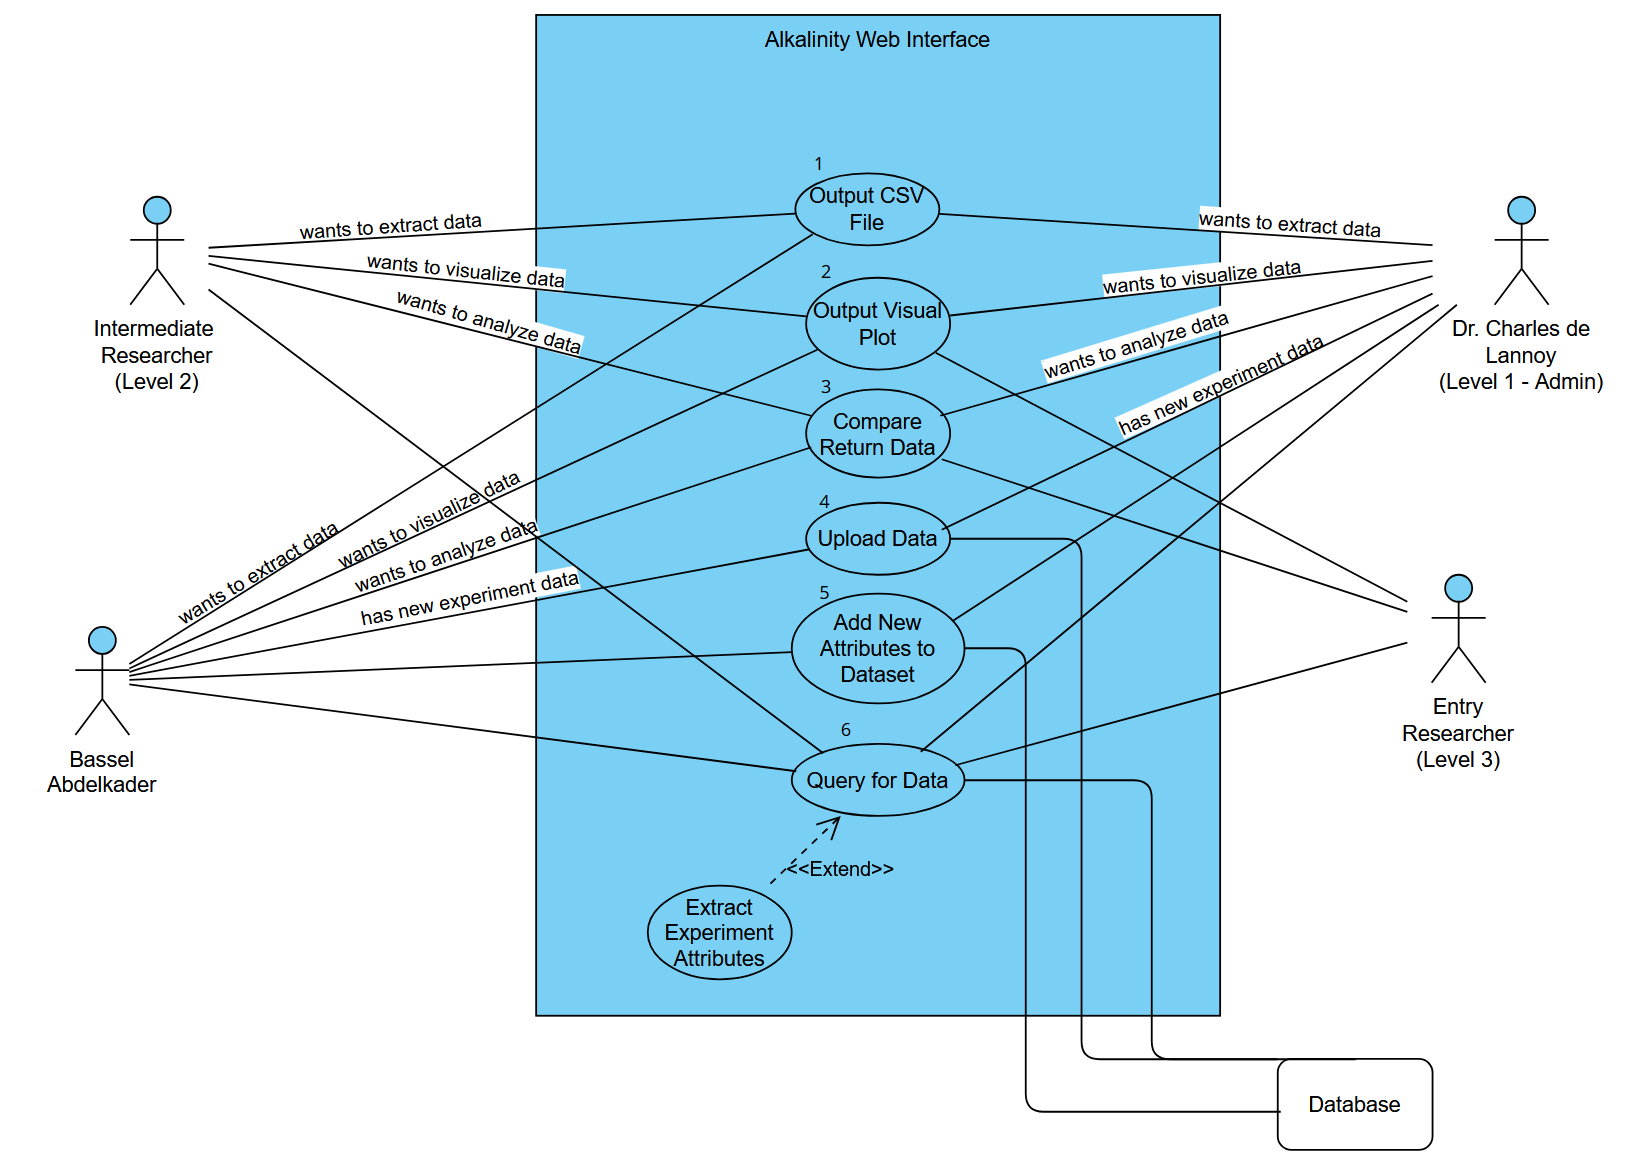
\includegraphics[scale=0.5]{capstoneUseCase.png}
\end{center}


\subsection{Product Use Case Table}
The product use case table (PUC) is an extention of the use case diagram in the pervious section. The table aims to provide more 
\begin{center}
  \begin{table}[]
    \centering
    \begin{tabular}{|p{0.08\linewidth}|p{0.3\linewidth}|l|p{0.4\linewidth}|}
      \hline
    \textbf{PUC No.} & \textbf{PUC Name} & \textbf{Actor/s} & \textbf{Input \& Output}\\
    \hline
    1 & Output CSV& \begin{tabular}[c]{@{}l@{}}Dr.\ Charles de Lannoy\\ Bassel Abdelkader\\ Intermediate Researcher\end{tabular} & \begin{tabular}[c]{@{}l@{}}Downloadable CSV file with\\ appropriate data (out)\\ Success or failure message\\ (out)\end{tabular}                                               \\
    \hline
    2 & Output Visual Plot & \begin{tabular}[c]{@{}l@{}}Dr.\ Charles de Lannoy\\ Bassel Abdelkader\\ Intermediate Researcher\\ Entry Researcher \end{tabular} & \begin{tabular}[c]{@{}l@{}}downloadable portable network\\ graphic (PNG) or portable\\ document format (PDF) file \\(out)\\ Online viewable plot graphic \\(out)\end{tabular}      \\
    \hline
    3 & Compare Return Data & \begin{tabular}[c]{@{}l@{}}Dr.\ Charles de Lannoy\\ Bassel Abdelkader\\ Intermediate Researcher\\ Entry Researcher \end{tabular} & \begin{tabular}[c]{@{}l@{}}Online viewable table of result \\(out)\\ Data analysis results of\\ involved data(out)\end{tabular}                                                \\
    \hline
    4 & Upload Data & \begin{tabular}[c]{@{}l@{}}Dr.\ Charles de Lannoy\\ Bassel Abdelkader\\ Database\end{tabular} & \begin{tabular}[c]{@{}l@{}}CSV file in expected format \\and attributes (in)\\ Success or failure user message \\(out)\\ Update database with inputted\\ data (out)\end{tabular} \\
    \hline
    5 & Add New Attributes to Dataset & \begin{tabular}[c]{@{}l@{}}Dr.\ Charles de Lannoy\\ Bassel Abdelkader\\ Database \end{tabular} & \begin{tabular}[c]{@{}l@{}}Update database with the new \\attribute (out)\\ Success or failure user message \\(out)\\ Attribute name of string type \\(in)\end{tabular}          \\
    \hline
    6 & Query for Data & \begin{tabular}[c]{@{}l@{}}Dr.\ Charles de Lannoy\\ Bassel Abdelkader\\ Intermediate Researcher\\ Entry Researcher\\ Database \end{tabular} & \begin{tabular}[c]{@{}l@{}}Visual online table with the \\queried data (out)\\ Selected attribute(s), dates,\\ restrictions (in)\end{tabular}\\
    \hline
    \end{tabular}
  \end{table}  
\end{center}

\newpage  \subsection{Individual Product Use Cases (PUC's)}
\subsubsection{Output CSV}
\begin{itemize}
  \item Description: The user can export/output the data that they have received
  from any function on the website system
  \item Pre-condition: There must be some data in the database. The information
  the user wants to output must also be able to be stored in a CSV file 
  \item Post-condition: The user will get to download the desired CSV file
  containing data from the database. If the download file has been sent to the
  system, the user will receive a success or failure message.
  \item Basic path: After querying the data from the database is successful, the
  user can click on the download CSV button to export the file onto their system.
\end{itemize}

\subsubsection{Output Visual Plot}
\begin{itemize}
  \item Description: The user is able to generate a graphical plot based on data
  from the database. The contents of the graph can be customized to include any
  sort of data that the user decides from the data base. The graph type can be determined by the user. 
  \item Pre-condition: There must be some selected data to be used to plot a graph.
  \item Post-condition: A online view of the plot will be generated and
  displayed on the website. There will also be an option for downloadable version. 
  \item Basic path: After querying the database for desired data, the user can
  pick the option to plot the returned data. The website will then generate a
  graphical plot based on the returned data.
\end{itemize}

\subsubsection{Compare Return Data}
\begin{itemize}
  \item Description: This use case will allow the user to compare two sets of
  data such as differences or similarities among other criteria.
  \item Pre-condition: There must be two sets of data and what attribute(s) are
  being compared. 
  \item Post-condition: The analysis of the data will be presented in a visual
  manner. Possible outcome may include colour coded elements or a small statement. 
  \item Basic path: After querying the database for desired data, the user can
  choose to enable the compare function. The user will then need to pick what
  attributes they would like to compare and then continue with the website
  prompts which will eventually give the data analysis result.
\end{itemize}

\subsubsection{Upload Data}
\begin{itemize}
  \item Description: When the user has more experimental data and would like to
  update the database, this function of the website will be used to take in the
  data and update/add to the existing database.
  \item Pre-condition: The file with the new data will be a CSV file and will
  need to be uploaded through the website interface.
  \item Post-condition: A success or failure message will be displayed to the
  user once the file is done uploading and have been added to the database.
  \item Basic path: The user will need to click on the upload data button and
  find the file they wish to upload on their system and upload it through the
  website's drop box. 
\end{itemize}
\subsubsection{Add New Attributes to Dataset}
\begin{itemize}
  \item Description: As the experiment and data become larger or changes have
  been made, there will be times when the dataset will need to be changed by
  adding new attributes.  
  \item Pre-condition: The user must specify which dataset that they want to
  edit. The user must then specify what is the attribute name is in the form of
  a string type input. 
  \item Post-condition: A success or failure message will be displayed to the
  user once the new attribute has been added to the database. 
  \item Basic path: The user will need to click on the edit dataset button. The
  user must then fill in the input fields with the correct information
\end{itemize}

\subsubsection{Query for Data}
\begin{itemize}
  \item Description: The user will want to get data from their past experiments.
  To do so, they will need to decide what they want. This is one of the main use
  case for any user/actor. 
  \item Pre-condition: The database must have the some data. The user's query
  request must be filled in through the input fields. The fields can range from
  dates, to strings, to constraints. 
  \item Post-condition: The returned data will be shown to the user through a
  visual table representation and will be presented with a range of other
  functions that the user can do with the returned data.  
  \item Basic path: The user will need to click on the query function button.
  They will then need to fill in the input fields, go through the user prompts
  to then get the output.
\end{itemize}

\section{Functional Requirements}
\subsection{Data Input Requirements}
  \begin{enumerate}
    \item[\textbf{FR-1.}] The system shall allow the user to input new
    experiment data or parameters.
    \begin{itemize}
    \item \textit{Rationale:} The system needs to be kept up-to-date with
    ongoing experiments, which may include new parameters that did not exist
    previously.
    \item \textit{Fit Criterion:} The user should be able to input new data and
    parameters with 0 errors.
    \end{itemize}
    \item[\textbf{FR-2.}] The system shall store experiment data in the database
    with all associated parameters and values correctly labelled.
    \begin{itemize}
      \item \textit{Rationale:} Ensures that data retrieval and analysis will be
      correct and accurate.
      \item \textit{Fit Criterion:} The system database parameters and values
      shall match the original experiment data parameters and values.
    \end{itemize}
  \end{enumerate}

\subsection{Data Migration and Organization Requirements}
  \begin{enumerate}
    \item[\textbf{FR-3.}] The system shall read existing experiment data stored
    in .CSV files.
    \begin{itemize}
      \item \textit{Rationale:} Existing experiment data is stored in Excel
      spreadsheets and must be integrated into the new system for continuity and
      analysis.
      \item \textit{Fit Criterion:} The system shall read and import the data
      files with 0 errors.
    \end{itemize}
    \item[\textbf{FR-4.}] The system shall organize experiment data by
    timestamps and experiment ID for unique identification.
    \begin{itemize}
      \item \textit{Rationale:} Each experiment needs to be separately
      identified for quick retrieval of data and efficiency in search or query
      actions.
      \item \textit{Fit Criterion:} Each ID and timestamp shall be traceable to
      one experiment.
    \end{itemize}
  \end{enumerate}

\subsection{Data Search and Query Requirements}
\begin{enumerate}
  \item[\textbf{FR-5.}] The system shall allow the user to search for specific
  datasets based on different parameters.
  \begin{itemize}
    \item \textit{Rationale:} Allows for quick look-ups of certain experiments
    and their results.
    \item \textit{Fit Criterion:} The system shall retrieve the correct
    experiments based on the matching parameters.
  \end{itemize}
  \item[\textbf{FR-6.}] The system shall allow the user to query two or more
  parameters or datasets for comparison and analysis.
  \begin{itemize}
    \item \textit{Rationale:} Allows for direct comparisons between different
    experiment parameters and/or results, which is necessary for analysis.
    \item \textit{Fit Criterion:} The system shall retrieve the correct
    parameters and/or experiments based on the query inputs.
  \end{itemize}
  \item[\textbf{FR-7.}] The system shall display the results of a user’s
  selected search or query in a format that is readable to the user.
  \begin{itemize}
    \item \textit{Rationale:} The user needs to see the results in a format that
    they can interpret.
    \item \textit{Fit Criterion:} The results shall be displayed in a table with
    all labels correct and legible.
  \end{itemize}
\end{enumerate}

\subsection{Data Visualization Requirements}
\begin{enumerate}
  \item[\textbf{FR-8.}] The system shall generate visual graphs based on
  selected parameters and datasets.
  \begin{itemize}
    \item \textit{Rationale:} Visual representation of the data allows for easy
    interpretation and graphical analysis.
    \item \textit{Fit Criterion:} The result should display a graphical plot
    with a title, axes, labels, and a legend.
  \end{itemize}
  \item[\textbf{FR-9.}] The system shall allow the user to customize the data
  visualization by adjusting axes, data ranges, labels, etc.
  \begin{itemize}
    \item \textit{Rationale:} Allows the user to adjust the graphical
    representation to their needs for their analysis.
    \item \textit{Fit Criterion:} Modifications to axes, data ranges, labels
    should be reflected in the generated graph in real-time.
  \end{itemize}
\end{enumerate}

\subsection{Data Analysis Requirements}
\begin{enumerate}
    \item[\textbf{FR-10.}] The system shall analyze patterns and trends in the
    experiment data based on the user’s selected parameters.
    \begin{itemize}
      \item \textit{Rationale:} Trend analysis is critical for the user to
      discover important findings pertaining to the experiment.
      \item \textit{Fit Criterion:} The system shall generate a result of the
      analysis to display to the user.
    \end{itemize}
    \item[\textbf{FR-11.}] The system shall use machine learning algorithms to
    predict and interpolate the data.
    \begin{itemize}
      \item \textit{Rationale:} Allows for future predictions of data and
      efficiency in running future experiments.
      \item \textit{Fit Criterion:} The system shall generate a report of value
      predictions or interpolate a graph and provide the interpolated data
      points.
    \end{itemize}
\end{enumerate}

\subsection{Error Tracking Requirements}
This section outlines functional requirements for one of the project's stretch
goals.
\begin{enumerate}
  \item[\textbf{FR-12.}] The system shall track and log errors in the experiment
  data.
  \begin{itemize}
    \item \textit{Rationale:} Helps users identify irrelevant or missing
    parameters.
    \item \textit{Fit Criterion:} Missing values from input data should be
    flagged.
  \end{itemize}
  \item[\textbf{FR-13.}] The system shall remove data logged as errors.
  \begin{itemize}
    \item \textit{Rationale:} Ensures data is organized and produce accurate
    results in analysis.
    \item \textit{Fit Criterion:} Flagged data should be removed from the
    database after user confirmation.
  \end{itemize}
\end{enumerate}

\subsection{User Access Management Requirements}
This section outlines functional requirements for one of the project's stretch
goals.
\begin{enumerate}
  \item[\textbf{FR-14.}] The system shall allow the user to sign in with valid
  credentials.
  \begin{itemize}
    \item \textit{Rationale:} Ensures the data can only be accessed and modified
    by authorized users.
    \item \textit{Fit Criterion:} The user shall be able to log in with a
    username and password.
  \end{itemize}
\end{enumerate}

\subsection{Data Export Requirements}
This section outlines functional requirements for one of the project's stretch
goals.
\begin{enumerate}
  \item[\textbf{FR-15.}] The system shall generate a report of queries in a
  session for the user to save or download.
  \begin{itemize}
    \item \textit{Rationale:} Allows user to keep a record of their findings for
    future use or reference.
    \item \textit{Fit Criterion:} The report should be exported in CSV or PDF
    format.
  \end{itemize}
\end{enumerate}

\section{Look and Feel Requirements}
This section will highlight the look and feel of the web interface for the
project involving the appearance and the style of the user interface and
experience.
\subsection{Appearance Requirements}
\begin{enumerate}
  \item[LFR-1.] The website should have a simple and organized layout, with
  clearly defined sections where all major functions should be easily accessible
  and viewable.
  \begin{itemize}
    \item \textit{Rationale:} Having a simple organized layout will ensure that the
    navigation of the website is quick and intuitive for accessing features and
    functions, which will enhance the user experience.
    \item \textit{Fit Criterion:} A user should be able to identify all the major
    functions of the website within five minutes of use.
  \end{itemize}
  
  \item[LFR-2.] The website shall be responsive on all computer and laptop screens
  aside from mobile screens.
  \begin{itemize}
    \item \textit{Rationale:} Having a responsive website will ensure that the
    application accommodates the majority, if not all, of the user base in having a
    proper user experience. 
    \item \textit{Fit Criterion:} The usability of the website should be the same
    as the default view on larger and smaller computer, laptop, and monitor screens.
  \end{itemize}
  
  \item[LFR-3.] The website's functions and buttons shall be properly labeled
  so that no button is ambiguous to users.
  \begin{itemize}
    \item \textit{Rationale:} Limiting ambiguity will ensure that users
    understand and recognize the functions to minimize confusion and improve
    efficiency.
    \item \textit{Fit Criterion:} A user should be able to tell what all buttons
    inherently do without needing to ask questions.
  \end{itemize}
  
  \item[LFR-4.] The produced plot from the data shall be properly labeled.
  \begin{itemize}
    \item \textit{Rationale:} Properly labeling plots will help users
    accurately interpret the data to make important analytical understandings.
    \item \textit{Fit Criterion:} The plots should not be ambiguous; users
    should be able to understand what the plot is about within five minutes of
    viewing it.
  \end{itemize}
\end{enumerate}


\subsection{Style Requirements}
\begin{enumerate}
  \item[LFR-5.] All icons on the website must be in the design standard. 
  \begin{itemize}
    \item \textit{Rationale:} To enforce an identity and unity for the website. 
    \item \textit{Fit Criterion:} After a user's first encounter with the product, 90\% of users should
    see that there is unity among all the icons on the website. 
  \end{itemize}
  
  \item[LFR-6.] All colors must match the theme of the website.
  \begin{itemize}
    \item \textit{Rationale:} Applying a theme will ensure users have
    an engaging visual experience.
    \item \textit{Fit Criterion:} After a user's first encounter with the product, 80\% of users
    should agree that there is a common theme throughout the website.
  \end{itemize}
  
  \item[LFR-7.] All fonts are to be consistent throughout the website. 
  \begin{itemize}
    \item \textit{Rationale:} Consistent fonts will increase readability,
    ensuring users can focus on the functionalities that matter on the page rather than inconsistencies. 
    \item \textit{Fit Criterion:} After a user's first encounter with the product, there should
    be no user who feels that any fonts do not belong on the website. 
  \end{itemize}
\end{enumerate}


\section{Usability and Humanity Requirements}
\subsection{Ease of Use Requirements}
\textbf{Description}: The product must be easy to navigate and use for
individuals with basic computer literacy.\\
\textbf{Rationale}: The product must be user-friendly. In the context of this
project, basic computer literacy is defined to encompass five computer skills -
using a keyboard to type, using a mouse to navigate, understanding basic
software applications such as word processing and spreadsheets, browsing the
internet, and managaing files and folders.\\ 
\textbf{Fit Criterion}: An individual with basic computer literacy must be able
to launch the application and upload an input file without any assistance from
the administrator.

\subsection{Personalization and Internationalization Requirements}
\textbf{Description}: The current version of the product will only be available
in English (EN-US) and more languages can be added in the later versions.\\
\textbf{Rationale}: Currently, the product is only expected to be used by
McMaster faculty and staff who are fluent in English.\\
\newline
\textbf{Description}: The product must recognize commonly used scientific and
mathematical symbols.\\
\textbf{Rationale}: The product shall be used to store scientific parameters as
datapoints so the product must be able to recognize commonly used symbols used
to specify scientific properties.\\
\textbf{Fit Criterion}: The product must be able to recognize the uppercase and
lowercase Greek Alphabet.

\subsection{Learning Requirements}
\textbf{Description}: Users must be able to use the product without any formal
training and with minimal guidance.\\
\textbf{Rationale}: The product shall be intuitive to use. Users must be able to
freely naviagte and experiment with the product after a simple product
walkthrough.\\
\textbf{Fit Criterion}: A new user with basic computer literacy skills should be
able to upload an input file, enter initial experiment parameters, select fields
to be compared and view their graph after a simple product walkthrough by the
administrator.

\subsection{Understandability and Politeness Requirements}
\emph{N/A}

\subsection{Accessibility Requirements}
\emph{N/A}

\section{Performance Requirements}
\subsection{Speed and Latency Requirements}
\begin{enumerate}
\item The system shall store new data or parameters within 60 seconds of input.
\item The system shall retrieve data from the database within 50ms for typical
search and queries.
\item The interaction between the interface and the user shall have a maximum
response time of 2 seconds.
\item The system shall have a maximum latency of 2 seconds for typical search
and queries.
\item The system shall generate a visualization of the data within 5 seconds.
\end{enumerate}
\begin{itemize}
  \item \textit{Rationale:} Quick response times ensure efficiency and smooth
  user experience without disrupting the flow of the user's thought processes.
  \item \textit{Fit Criterion:} The system shall satisfy the requirements above.
\end{itemize}

\subsection{Safety-Critical Requirements}
The product does not have safety-critical requirements to consider.

\subsection{Precision or Accuracy Requirements}
\begin{enumerate}
  \item All parameter values shall be accurate to four decimal places.
  \item All timestamps of experiment data shall be accurate to milliseconds. 
  \item Values on visual data plots shall be accurate to four decimal places.
\end{enumerate}
\begin{itemize}
  \item \textit{Rationale:} Accuracy of the data is critical for data analysis,
  prediction, and interpolation.
  \item \textit{Fit Criterion:} The system shall satisfy the requirements above.
\end{itemize}

\subsection{Robustness or Fault-Tolerance Requirements}
\begin{enumerate}
  \item The application shall not terminate but display an error message if it
  loses connection to the backend server.
  \item The application shall provide basic functionality if it loses connection
  to the internet.
\end{enumerate}
\begin{itemize}
  \item \textit{Rationale:} The system should not fail or crash when
  experiencing unexpected circumstances.
\end{itemize}

\subsection{Capacity Requirements}
\begin{enumerate}
  \item The application shall allow for up to three simultaneous users.
  \item The system shall store up to x amount of data.
\end{enumerate}
\begin{itemize}
  \item \textit{Rationale:} The system must be capable of storing and processing
  large amounts of data.
  \item \textit{Fit Criterion:} The system shall satisfy the requirements above.
\end{itemize}

\subsection{Scalability or Extensibility Requirements}
\begin{enumerate}
  \item The system shall be able to process and store the existing data. The
  amount of data going into the system is expected to grow until the experiment
  study comes to an end.
  \item The system shall be able to add additional parameters that did not
  previously exist in the database at the discretion of the user.
\end{enumerate}
\begin{itemize}
  \item \textit{Rationale:} The system must be able to expand to keep up with
  future experiments.
\end{itemize}

\subsection{Longevity Requirements}
\begin{enumerate}
  \item The system shall operate for the duration of the experiment study.
\end{enumerate}

\section{Operational and Environmental Requirements}
\subsection{Expected Physical Environment}
\begin{enumerate}
  \item The application shall operate in a typical office environment with
  reliable internet connectivity.
  \item The application shall be compatible with a desktop or laptop
  environment.
\end{enumerate}
\begin{itemize}
  \item \textit{Rationale:} Ensures functionality in environments where
  end-users are most likely to use the application, accomodating several screen
  sizes and operating systems. 
  \item \textit{Fit Criterion:} Testing will be conducted on the two most common
  operating systems, Windows and macOS.
\end{itemize}

\subsection{Wider Environment Requirements}
\lips

\subsection{Requirements for Interfacing with Adjacent Systems}
\begin{enumerate}
  \item The application shall operate on the most recent versions of Google
  Chrome and Apple Safari.
\end{enumerate}
\begin{itemize}
  \item \textit{Rationale:} The application must be able to operate on these two
  most common web browsers, as these will be the primary platforms where it is
  hosted and accessed by users.
  \item \textit{Fit Criterion:} Performance testing shall be done to ensure the
  application functions correctly.
\end{itemize}

\subsection{Productization Requirements}
\begin{enumerate}
  \item The system shall be distributed as a web application.
  \item The system shall have an easy onboarding process with user
  documentation.
  \begin{itemize}
    \item \textit{Rationale:} Ensures that users can use the application without
    needing frequent support.
    \item \textit{Fit Criterion:} Usability testing shall be done to ensure
    users are able to onboard easily.
  \end{itemize}
\end{enumerate}

\subsection{Release Requirements}
\begin{enumerate}
  \item The first version of the system shall be released after project
  completion.
\end{enumerate}

\section{Maintainability and Support Requirements}
Maintenance requirements encompass the strategies and processes needed to ensure
a system remains functional, efficient, and up-to-date throughout its lifecycle.

\subsection{Maintenance Requirements}
\begin{enumerate}
  \item[\textbf{MSR-1.}] The application’s maintenance must be the
  responsibility of the development team with no involvement from the users.
  \begin{itemize}
    \item \textit{Rationale:} Ensures that skilled personnel handle maintenance.
  \end{itemize}

  \item[\textbf{MSR-2.}] Documentation must be provided to be referenced for
  future maintenance and to enable seamless knowledge transfer to a new team.
  \begin{itemize}
    \item \textit{Rationale:} Ensures smooth onboarding and continuity in
    development.
    \item \textit{Fit Criterion:} The documentation must be updated with every
    major release.
    \item \textit{Traceability:} MSR-3.
  \end{itemize}

  \item[\textbf{MSR-3.}] The application must be designed to accommodate future
  development, including the addition of new experimental parameters or features
  without backwards progression.
  \begin{itemize}
    \item \textit{Rationale:} Ensures the application can scale and evolve
    without compromising existing features.
    \item \textit{Traceability:} FR-4, FR-12, MSR-2.
  \end{itemize}
\end{enumerate}

\subsection{Supportability Requirements}
\begin{enumerate}
  \item[\textbf{MSR-4.}] 
  The application must have an intuitive user interface that allows users to
  operate it independently without requiring external assistance.
  \begin{itemize}
    \item \textit{Rationale:} Ensures a user-friendly experience that reduces
    the need for help desk support.
    \item \textit{Fit Criterion:} At least 90\% of users should be able to
    complete tasks without needing support.
    \item \textit{Traceability:} LF-1, LF-2, LF-3, UHR-1, UHR-4.
  \end{itemize}

  \item[\textbf{MSR-5.}] The application must have automated guidance, such as
  error messages, to assist users in troubleshooting common issues.
  \begin{itemize}
    \item \textit{Rationale:} Ensures users can resolve issues on their own,
    reducing the volume of support requests.
    \item \textit{Fit Criterion:} The documentation must be updated with every
    major release and reviewed quarterly to ensure accuracy.
    \item \textit{Traceability:} FR-12.
  \end{itemize}
\end{enumerate}

\subsection{Adaptability Requirements}
\begin{enumerate}
  \item[\textbf{MSR-6.}] The application must be compatible with modern web
  browsers to ensure widespread accessibility.
  \begin{itemize}
    \item \textit{Rationale:} Ensures the application is accessible to a broad
    range of users and devices.
    \item \textit{Fit Criterion:} The application should at least be able to run
    on the latest version of Chromium-based web browsers.
    \item \textit{Traceability:} LF-1, LF-2.
  \end{itemize}
\end{enumerate}
\section{Security Requirements}
Security requirements focus on protecting data, controlling access, ensuring
integrity, and auditing user actions within the application.

\subsection{Access Requirements}
\begin{enumerate}
  \item[\textbf{SR-1.}] Access to the application must be restricted to
  authorized personnel, with an authentication mechanism.
  \begin{itemize}
    \item \textit{Rationale:} Ensures that only authorized users can interact
    with the application.
    \item \textit{Fit Criterion:} Only users with valid credentials should
    access the application.
    \item \textit{Traceability:} FR-14, SR-2, SR-8, SR-10.
  \end{itemize}

  \item[\textbf{SR-2.}] Only authenticated users should have the ability to
  query or modify the data, and each user’s access must be limited to their
  capabilities within the application.
  \begin{itemize}
    \item \textit{Rationale:} Ensures users can only perform actions that align
    with their roles.
    \item \textit{Fit Criterion:} The application should restrict 100\% of
    actions that are not permitted to the user's level of access.
    \item \textit{Traceability:} FR-14, SR-1, SR-8.
  \end{itemize}
\end{enumerate}

\subsection{Integrity Requirements}
\begin{enumerate}
  \item[\textbf{SR-3.}] The application must validate data inputs to ensure they
  conform to expected formats and values before they are processed.
  \begin{itemize}
    \item \textit{Rationale:} Ensures only valid data is processed, reducing
    errors.
    \item \textit{Fit Criterion:} 100\% of inputs must pass validation checks
    before processing.
    \item \textit{Traceability:} FR-1, FR-2, FR-4.
  \end{itemize}

  \item[\textbf{SR-4.}] The application must not modify the data unnecessarily
  through its transfer process.
  \begin{itemize}
    \item \textit{Rationale:} Ensures the original data remains accurate and
    unaltered.
    \item \textit{Fit Criterion:} Data should remain unchanged unless explicitly
    modified, with logs confirming its integrity.
    \item \textit{Traceability:} FR-3, FR-4, SR-5, SR-6.
  \end{itemize}

  \item[\textbf{SR-5.}] The application must ensure that any data processed or
  transferred is free from duplication or inconsistencies.
  \begin{itemize}
    \item \textit{Rationale:} Ensures data consistency and prevents corruption.
    \item \textit{Fit Criterion:} The application must detect and prevent 100\%
    of duplicated records.
    \item \textit{Traceability:} FR-3, FR-4, SR-4, SR-6.
  \end{itemize}

  \item[\textbf{SR-6.}] The application must have safeguards in place to
  maintain the accuracy of the transferred data.
  \begin{itemize}
    \item \textit{Rationale:} Ensures reliable data transfer without loss or
    error.
    \item \textit{Fit Criterion:} Transfer operations should maintain 100\% data
    accuracy, verified by validation tests.
    \item \textit{Traceability:} FR-3, FR-4, SR-4, SR-5.
  \end{itemize}
\end{enumerate}

\subsection{Privacy Requirements}
\begin{enumerate}
  \item[\textbf{SR-7.}] All personal information related to experimental
  participants or stakeholders, if applicable, must be anonymized and handled in
  accordance with relevant privacy laws and regulations.
  \begin{itemize}
    \item \textit{Rationale:} Ensures user privacy and legal compliance.
    \item \textit{Traceability:} SR-8.
  \end{itemize}

  \item[\textbf{SR-8.}] The application must restrict data sharing with external
  parties unless expressly authorized by stakeholders, and users must be fully
  informed about the privacy policies.
  \begin{itemize}
    \item \textit{Rationale:} Ensures transparency and control over data
    sharing.
    \item \textit{Traceability:} FR-14, SR-1, SR-2, SR-7.
  \end{itemize}
\end{enumerate}

\subsection{Audit Requirements}
\begin{enumerate}
  \item[\textbf{SR-9.}] The application must maintain a comprehensive audit
  trail, logging all access and modification events, including timestamps and
  identities of users performing actions.
  \begin{itemize}
    \item \textit{Rationale:} Ensures accountability and traceability of
    actions.
    \item \textit{Fit Criterion:} 100\% of data access and modification events
    must be logged and retrievable.
    \item \textit{Traceability:} FR-12, FR-13.
  \end{itemize}

  \item[\textbf{SR-10.}] Audit logs must be securely stored and accessible only
  by authorized personnel.
  \begin{itemize}
    \item \textit{Rationale:} Ensures the security and integrity of audit data.
    \item \textit{Fit Criterion:} Logs must be encrypted and accessible only to
    users with administrative privileges.
    \item \textit{Traceability:} FR-14, SR-1.
  \end{itemize}
\end{enumerate}

\subsection{Immunity Requirements}
\begin{enumerate}
  \item[\textbf{SR-11.}] The application must have proactive measures to detect
  and mitigate suspicious activities, such as repeated unauthorized access
  attempts, ensuring the application remains secure at all times.
  \begin{itemize}
    \item \textit{Rationale:} Ensures early detection and prevention of security
    breaches.
    \item \textit{Fit Criterion:} The application must detect and block
    unauthorized attempts after three failed login attempts, with automated
    alerts sent to administrators.
    \item \textit{Traceability:} FR-14.
  \end{itemize}
\end{enumerate}

\section{Cultural Requirements}
\subsection{Cultural Requirements}
\lips

\section{Compliance Requirements}
\subsection{Legal Requirements}
\lips
\subsection{Standards Compliance Requirements}
\lips

\section{Open Issues}
\lips
\section{Off-the-Shelf Solutions}

Off-the-shelf solutions are evaluated to explore whether existing products can
meet the project’s needs or if custom development is required. By comparing
available options, the team can determine which aspects of these products
satisfy the project's requirements while also identifying their limitations.

\subsection{Ready-Made Products}

Products that could meet most or all of the project’s requirements without
significant customization:

\begin{itemize}
    \item \textbf{Microsoft Power BI}: A business analytics tool capable of
    handling large datasets, offering data import from CSV files and advanced
    visualizations.
    
    \begin{itemize}
        \item \textbf{Key Features:}
        \begin{itemize}
            \item Supports CSV imports and data querying.
            \item Scalable data handling.
            \item Generates dynamic visualizations.
        \end{itemize}

        \item \textbf{Limitations:}
        \begin{itemize}
            \item High-cost licensing for continuous use.
            \item Real-time CSV data updates might be challenging to implement.
            \item Lacks flexibility for scientific applications, especially
            niche inter-parameter comparability.
        \end{itemize}
    \end{itemize}

    \item \textbf{Tableau}: A data visualization tool known for creating
    interactive dashboards from large datasets.
    
    \begin{itemize}
        \item \textbf{Key Features:}
        \begin{itemize}
            \item Powerful querying.
            \item Generates dynamic visualizations.
            \item Interactive dashboards with advanced analytics.
        \end{itemize}

        \item \textbf{Limitations:}
        \begin{itemize}
            \item High-cost licensing for continuous use.
            \item Lacks support for scientific-specific customization.
            \item Not designed for handling algorithmic data comparisons or
            extending to new experimental parameters.
        \end{itemize}
    \end{itemize}
\end{itemize}

\subsection{Reusable Components}

Products that could be used by the project.


\begin{itemize}
    \item \textbf{D3.js}: A JavaScript library for creating dynamic, interactive
    visualizations.
    
    \begin{itemize}
        \item \textbf{Key Features:}
        \begin{itemize}
            \item Highly customizable for complex data visualizations.
            \item Integrates with web technologies (e.g., React).
        \end{itemize}
    \end{itemize}

    \item \textbf{Plotly.js}: A JavaScript library for building interactive
    plots and graphs in web applications.
    
    \begin{itemize}
        \item \textbf{Key Features:}
        \begin{itemize}
            \item Customizable graphs and charts for web interfaces.
            \item Supports real-time updates.
        \end{itemize}
    \end{itemize}
\end{itemize}


\subsection{Products That Can Be Copied}
N/A; no product exists that fits all the requirements out-of-the-box.


\section{New Problems}
\subsection{Effects on the Current Environment}
\lips
\subsection{Effects on the Installed Systems}
\lips
\subsection{Potential User Problems}
\lips
\subsection{Limitations in the Anticipated Implementation Environment That May
Inhibit the New Product}
\lips
\subsection{Follow-Up Problems}
\lips
\section{Tasks}
The team will follow an effective task management plan that emphasizes
structure, iterative progress, milestone tracking, and accountability for
successful project outcomes. 
\subsection{Project Planning}

The team will adopt an agile lifecycle approach, focusing on iterative progress
and adaptability. Work will be organized into stages, milestones, and phases,
with regular reviews and adjustments to ensure alignment with goals. Issues are
managed via GitHub and all communications are documented to ensure
accountability. Stakeholder feedback will be integrated throughout the process
to ensure the solution meets evolving requirements.

In addition, project planning will include weekly team meetings, biweekly
supervisor meetings. Deliverables are categorized into stages where roles are
rotated among team members to share responsibility.

\subsection{Planning of the Milestones}

The milestones provide a structured approach to the project's documentation,
planning, and demonstration activities. By the deadlines, the team is expected
to complete and review the documents to ensure accuracy, compliance with project
requirements, and readiness for subsequent stages.

\newpage
\begin{table}[htbp]
  \centering
  \begin{tabular}{|l|l|l|}
  \hline
  \textbf{Stage} & \textbf{Milestone} & \textbf{Deadline} \\
  \hline
  Stage 1 & Problem Statement, POC Plan, Development Plan & Sept 24 \\
  \texttt{} & Requirements Document Revision 0 & Oct 9 \\
  \hline
  Stage 2 & Hazard Analysis & Oct 23 \\
  \texttt{} & V\&V Plan Revision 0 & Nov 1 \\
  \hline
  Stage 3 & POC Demonstration & Nov 11 - 22 \\
  \hline
  Stage 4 & Design Document Revision 0 & Jan 15 \\
  \hline
  Stage 5 & Revision 0 Demonstration & Feb 3 - 14\\
  \hline
  Stage 6 & V\&V Report Revision 0 & Mar 7 \\
  \hline
  Stage 7 & Final Demonstration (Revision 1) & Mar 24 - 30\\
  \texttt{} & EXPO Demonstration & Apr TBD \\
  \texttt{} & Final Documentation (Revision 1) & Apr 2 \\
  \hline
  \end{tabular}
  \caption{Project Decomposition and Deadlines}
  \label{table:2}
\end{table}

\subsection{Planning of the Development Phases}

The development phases outline the progression of the project's coding and
implementation efforts. Each phase is focused on achieving significant technical
progress that works alongside the milestones to allow for incremental progress
and continuous refinement.

\newpage
\begin{table}[htbp]
  \centering
  \begin{tabular}{|l|l|l|}
  \hline
  \textbf{Stage} & \textbf{Milestone} & \textbf{Deadline} \\
  \hline
  Phase 1 & Backend Database Development & Nov 1 \\
  \texttt{} & Data Migration Algorithm & Nov 8 \\
  \texttt{} & POC Functional Testing & Nov 10 \\
  \texttt{} & POC Demonstration & Nov 11 \\
  \hline
  Phase 2 & Backend Refinement \& Bug Fixes & Dec 6 \\
  \texttt{} & Basic Frontend Development & Jan 3 \\
  \texttt{} & Frontend-Backend Integration & Jan 17 \\
  \texttt{} & Preliminary Testing \& Bug Resolution & Jan 24 \\
  \texttt{} & Revision 0 Demonstration & Feb 3 \\
  \hline
  Phase 3 & Final Frontend Features Development & Feb 14 \\
  \texttt{} & Backend Optimization & Feb 21 \\
  \texttt{} & Full System Testing \& Debugging & March 21 \\
  \texttt{} & Revision 1 Final Demonstration & March 24 \\
  \hline
  \end{tabular}
  \caption{Project Development Phases and Deadlines}
\end{table}

\noindent\textbf{Phase 1} focuses on the Proof of Concept (POC), where the team
is expected to develop and present a functional prototype that demonstrates the
core features and feasibility of the project. This phase focuses on the backend,
including building a database capable of querying and sorting data, and
implementing an algorithm to transfer data from a CSV file into the database
format.\newline\newline
\noindent\textbf{Phase 2} involves the Revision 0 Demonstration, where the
backend is expected to be fully completed according to the project requirements.
In addition, a basic frontend will be developed and integrated into a website to
allow interaction with the backend functionality. It is expected that some bugs
or issues will be displayed. \newline\newline
\noindent\textbf{Phase 3} Phase 3 is the Revision 1 Final Demonstration, where
the final version of the project is presented. During this phase, final frontend
features will be developed to improve the user interface. The backend will be
optimized for performance. Full system testing and debugging will address any
outstanding issues.  This phase represents the culmination of all development
efforts, with a fully functioning product that meets all requirements.
Ultimately, it highlights the project's readiness for production.


\section{Migration to the New Product}
\subsection{Requirements for Migration to the New Product}
\textbf{Q}: Will you use a phased implementation to install the new system? if
so, describe which requirements will be implemented by eahc of the major
phases?\\
\textbf{A}: No, the system will be installed in a single go after being tested
and approved.\\
\emph{Note}: Include cross-references between development tasks, project phases
and the Product Use Cases and atomic requirements.\\
\newline
\textbf{Q}: What kind of data conversion is necessary? Must special programs be
written to transport data from an existing system to a new one? If so, describe
the requirements for these programs here.\\
\textbf{A}: Currently, the files are stored in the CSV format. In order to make
them compatiable for migration to the new database (MongoDB), the files must be
converted into JavaScript Object Notaion (JSON) format. Yes, a special program
must be written to transport the data as the new system will only accept JSON
files. This means that when the file is inputted to the new system (in CSV
format), a special program must first convert it to JSON so that the data can be
entered in the database.\\
\newline
\textbf{Q}: What kind of manual backup is needed while the new system is
installed?\\
\textbf{A}: The installation of the new program should not be a long process and
can be accomplished on a day when there are no experiments being run in the lab.
This means, no manual backup would be necessary while the new system is being
installed.\\
\newline
\textbf{Q}: When are each of the major components to be put in place? When are
the phases of the implementation to be released?\\
\textbf{A}: No phases of implementation to be released. Major components will be
put in place based on this timeline - 
\begin{itemize}
  \item Database with migrated data and funtionality to compare parameters:
  Proof of Concept Demonstration
  \item Interface that allows inputting data and adding new parameters: End of
  December (before Christmas break)
  \item Dashboard that allows analysis of data and visualizing graphs: End of
  January 
\end{itemize}
\ \\
\textbf{Q}: Is there a need to run the new product in parallel with the existing
product?\\
\textbf{A}: No, there is no need to run the new product in parallel with the
existing product. Data can be migrated at regular intervals once the database is
up and running.\\
\newline
\textbf{Q}: Is there any special effort needed to decomission the old product?\\
\textbf{A}: The old product is essentially a collection of spreadsheets so no
special effort is needed to decomission them. A visual inspection and testing
might be required after data is migrated to the new product to ensure the
accuracy and integrity of the data.

\subsection{Data That Has to be Modified or Translated for the New System}
\textbf{Q}: Description of current technology that holds data.\\
\textbf{A}: Currently the data is retreived in the form of CSV files and copied
onto existing Excel templates that are used to sort and analyse the data.
Although the templates are sophisticated and well-deisgned, a lot of manual work
is involved to flag incorrect data (rows of zeroes for all parameters), remove
redundant data (the data file is sometimes split into multiple CSV files that
might contain some overlapping data) and more.\\
\newline
Some of the collected paramteric data is also inaccurate (such as the power
voltage and density module) and so those columns of data are ignored. To compare
different experiments, the user is required to switch between experiment files
to view their respective graphs. This is cumbersome and as the number of
experiments increase, unsustainable in the long-term.\\
\newline
\textbf{Q}: Description of data translation tasks.\\
\textbf{A}: A scirpt will be written to automate the translation of files from
CSV to JSON format.\\
\newline
\textbf{Q}: Foreseeable Problems.\\
\textbf{A}: N/A

\section{Costs}
\lips
\section{User Documentation Requirements}
User documentation will cover the more complicated features and functionalities of the website.\\

\noindent This documentation will include how to add new attributes to the dataset, how
to request data plots and any major functionality features. \newline
This document is intended to be a help/tutorial for the end users who will be
using the site for its functionalities. Its target is for those who have limited
software knowledge. Although most functions aims to be as intuitive as possible
to the user, since this is an analysis application there should be documentation
explaining for those who have no idea about how research data works and how to
interact with it using the website.

\subsection{Training Requirements}
No training is required to use the end product. 

\section{Waiting Room}
The following requirements are beyond the sophistication of, or time allowed
for, initial release of the product.
\subsection{Automatically Download Data from Lab Apparatus}
\textbf{Description}: The product shall automatically download the CSV data
files from the lab apparatus and after conversion, upload them to the
database.\\
\textbf{Rationale}: Currently, the data has to be manually exported from the
machine at the end of every week to ensure that the data does not get lost or
overwritten.\\
\textbf{Expected Version}: Version 2

\subsection{Dynamic Dashboard to Generate Comparison Reports}
\textbf{Description}: The product shall include a dashboard that hosts multiple
visual plots that are dynamically updated based on changes in the data.\\
\textbf{Rationale}: For the initial release, only basic plots that are already
being used by the user will be available for viewing. Whenever data is modified,
the graph must be regenerated to view the updated plot.\\
\textbf{Expected Version}: Version 2

\subsection{Machine Learning Analysis and Projections}
\textbf{Description}: The product shall use machine learning algorithms to
automatically compare parameters and generate visual graphs based on simple text
prompts.\\
\textbf{Rationale}: The idea is to use artificial intelligence to suggest
parametric comparisons or visual graphs that the user might not have though of.
The aim is to explore analyses that might not have been considered by a user.\\
\textbf{Expected Version}: Version 3

\subsection{Mobile Development and Accessibility}
\textbf{Description}: The product shall comply with relevant accessibility
standards both for the web version and the mobile version.\\
\textbf{Rationale}: The project can be extended to include a mobile application
version of the product to increase accessibility and reachability.\\
\textbf{Expected Version}: Version 4

\section{Ideas for Solution}
\lips

\newpage{}
\section*{Appendix --- Reflection}

The information in this section will be used to evaluate the team members on the
graduate attribute of Lifelong Learning.  Please answer the following questions:

\begin{enumerate}
  \item What knowledge and skills will the team collectively need to acquire to
  successfully complete this capstone project?  Examples of possible knowledge
  to acquire include domain specific knowledge from the domain of your
  application, or software engineering knowledge, mechatronics knowledge or
  computer science knowledge.  Skills may be related to technology, or writing,
  or presentation, or team management, etc.  You should look to identify at
  least one item for each team member.
  \item For each of the knowledge areas and skills identified in the previous
  question, what are at least two approaches to acquiring the knowledge or
  mastering the skill?  Of the identified approaches, which will each team
  member pursue, and why did they make this choice?
\end{enumerate}

\end{document}